%!TEX program = xelatex
% 完整编译: xelatex -> biber/bibtex -> xelatex -> xelatex
\documentclass[lang=cn,11pt,a4paper]{elegantpaper}
\usepackage{enumitem}
\usepackage{booktabs}
\usepackage{diagbox} % for creating diagonal split in table cells
\usepackage{appendix}
\usepackage{pdfpages}
\usepackage{listings}
\usepackage{xcolor} % For color customization (optional)
\usepackage{hyperref}
\usepackage{biblatex}
\usepackage{float} % 使用float包以便使用H选项

\addbibresource{references.bib}


\title{自动增益控制放大器}
\date{\zhtoday}

\bibliography{references}


% 本文档命令
\usepackage{array}
\newcommand{\ccr}[1]{\makecell{{\color{#1}\rule{1cm}{1cm}}}}

\begin{document}
% Customizing the listings
\lstset{ %
  language=C,                % Choose the language of the code
  basicstyle=\ttfamily\small, % Set the font style and size
  keywordstyle=\color{blue},  % Color for keywords
  commentstyle=\color{gray},  % Color for comments
  stringstyle=\color{red},    % Color for strings
  numbers=left,               % Line numbers on the left
  numberstyle=\tiny\color{gray}, % Style for line numbers
  stepnumber=1,               % Line number interval
  numbersep=5pt,              % Space between line numbers and code
  backgroundcolor=\color{lightgray!20}, % Background color for the code
  showspaces=false,           % Don't show spaces
  showstringspaces=false,     % Don't show spaces in strings
  showtabs=false,             % Don't show tabs
  frame=single,               % Frame around the code
  tabsize=4,                  % Tab size
  captionpos=b,               % Caption position (b for bottom)
  breaklines=true,            % Line breaking
  breakatwhitespace=true,     % Break at whitespace
}
\maketitle

\begin{abstract}
  本文实现了一种自动增益控制放大器的设计和实现。通过方案论证,我们选择了基于数字电位器的AGC电路方案,该方案在电路结构和调节方面具有明显优势。硬件设计包括运算放大器、有效值检波电路、数字电位器、ADC采样模块、MCU和显示屏的选型与设计等。软件设计部分详细介绍了AD采样、数字电位器调节以及主程序的编写等。系统测试表明,所设计的自动增益控制系统在不同输入信号条件下均能保持良好的性能,满足设计要求。在测试过程中,我们也发现了信号源准确性和电路共地问题对系统性能的影响。最终,本设计验证了其可靠性和稳定性,为自动增益控制领域提供了一种有效的解决方案。
  
  本文完全采用\LaTeX{}书写,工程细节和完整代码见 GitHub: \url{https://github.com/wanansu/AGC_digital_potentiometer}
  \keywords{自动增益控制放大器(AGC),数字电位器,运算放大器,有效值检波电路,ADC采样,STM32单片机}
\end{abstract}

\section{方案论证}

\subsection{方案一: 运算放大器结合倒T型DAC电阻网络}

使用运算放大器结合倒T型数字模拟转换器(DAC)电阻网络来实现自动增益控制(AGC)电路。该方案的核心是通过数字信号控制倒T型DAC电阻网络的等效电阻,从而调节运算放大器的增益。输入信号接入运算放大器的输入端,输出信号通过反馈电阻网络回馈到反相输入端,以实现所需增益。设计信号检测电路,通过模数转换器(ADC)和STM32单片机实时监测和调整输入信号的幅度。

如图\ref{fig:DAC_net}所示,为使用multisim进行的运算放大器结合倒T型DAC电阻网络的电路仿真图。
\begin{figure}[!htb]
  \centering
  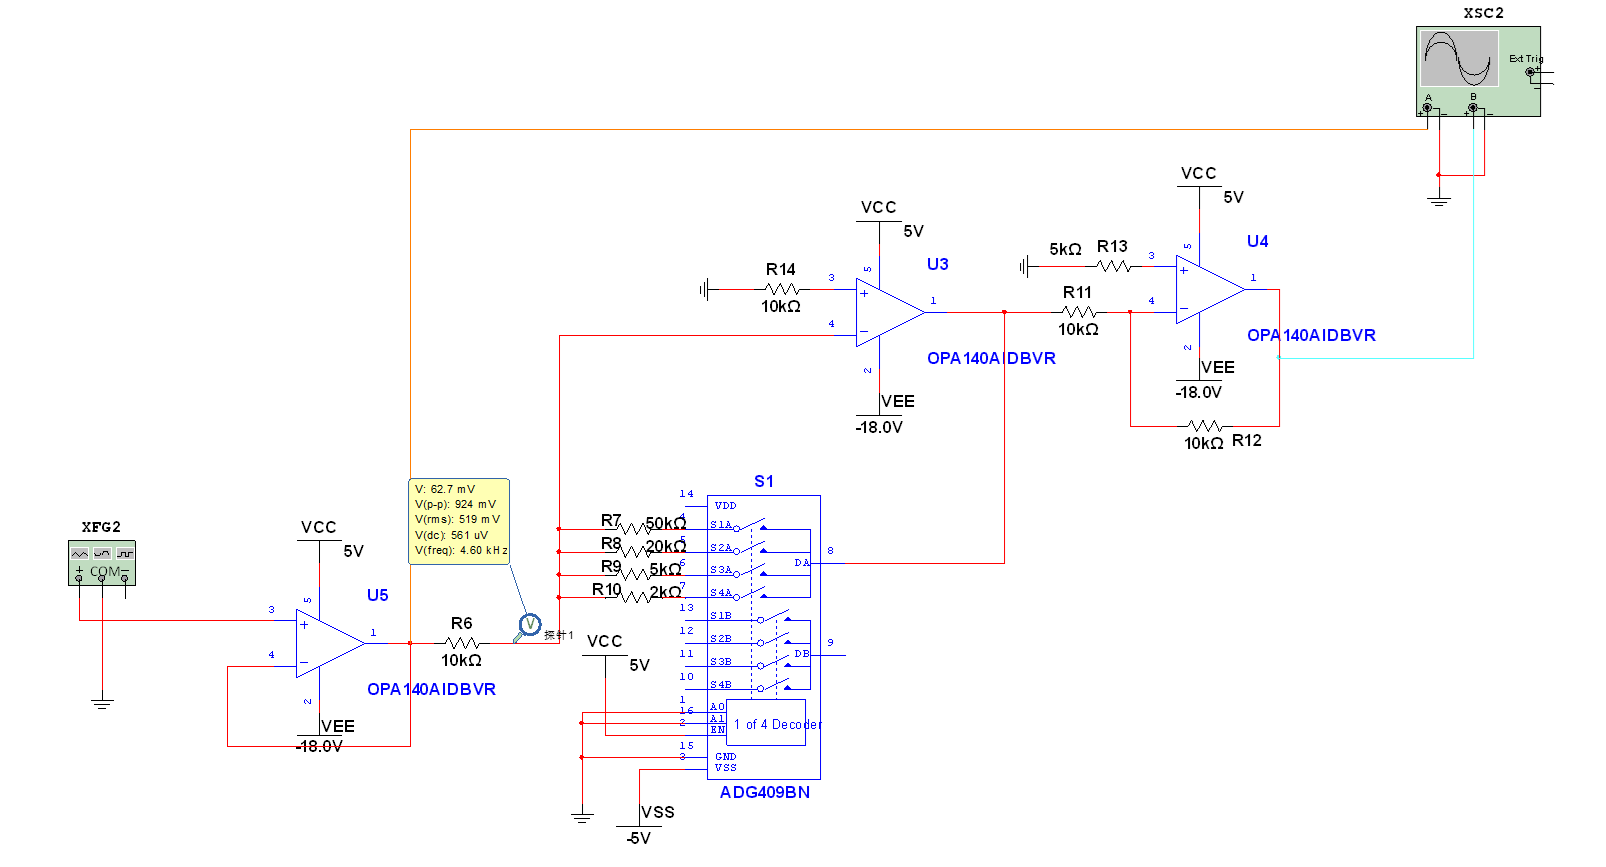
\includegraphics[width=1\textwidth]{DAC电阻网络.png}
  \caption{运算放大器结合倒T型DAC电阻网络 - mustisim仿真}
  \label{fig:DAC_net}
\end{figure}

\begin{itemize}
  \item 优点
        \begin{itemize}
          \item \textbf{原理简单:} 运算放大器和DAC电阻网络结合,原理易于理解。
          \item \textbf{可调性强:} 通过数字控制DAC电阻网络,实现精确的增益调节。
        \end{itemize}

  \item  缺点
        \begin{itemize}
          \item \textbf{电路复杂度高:} 需要设计复杂的DAC电阻网络,增加了电路设计难度。
          \item \textbf{控制难度大:} STM32对电路的控制需要精确的数字控制,调试和校准较为复杂。
        \end{itemize}
\end{itemize}
\subsection{方案二: 基于VCA821的AGC电路}

采用基于VCA821的AGC电路。VCA821是一款直流耦合、宽带、dB线性的压控增益放大器。将VCA821与OPA695后级放大器组合,输出信号再经过OPA820积分器,连接至VCA821的增益控制(VG)引脚,形成闭环,从而保证输出信号的稳定性。

如图\ref{fig:vca_agc}为使用TI公司的电路仿真软件Tina进行的基于VCA821设计的AGC电路仿真图:
\begin{figure}[!htb]
  \centering
  \includegraphics[width=1\textwidth]{VCA821的AGC1.jpg}
  \caption{基于VCA821的AGC电路 - Tina仿真}
  \label{fig:vca_agc}
\end{figure}

\begin{itemize}
  \item 优点
        \begin{itemize}
          \item \textbf{原理清晰:} VCA821的特性直观,增益可由外部控制引脚调节。
          \item \textbf{频率响应好:} 适用于宽带信号处理,输出信号稳定性高。
        \end{itemize}

  \item 缺点
        \begin{itemize}
          \item \textbf{电路复杂度高:} VCA821和其配套电路较为复杂,需要精确匹配和调试。
          \item \textbf{输入信号范围限制:} VCA821的输入信号范围可能不满足特定应用需求,需额外考虑信号处理。
        \end{itemize}
\end{itemize}

\subsection{方案三: 基于数字电位器的AGC电路}

采用基于数字电位器的AGC电路。设计一个两级反相放大电路,通过数字电位器调节电路的放大倍数,使用STM32单片机控制数字电位器,实现自动增益调节。对于交流信号,使用有效值检波电路将其转换为直流信号。利用ADC模块采集直流信号,通过单片机处理,实现对输入信号与输出信号的精确测量和调节。

\begin{itemize}
  \item  优点
        \begin{itemize}
          \item \textbf{电路结构简单:} 两级反相放大电路和数字电位器组成的调节电路结构清晰简单。
          \item \textbf{调节方便:} 通过STM32单片机控制数字电位器,调节方便快捷。
        \end{itemize}

  \item 缺点
        \begin{itemize}
          \item \textbf{噪声和干扰:} 数字电位器和其他数字元件可能引入噪声和干扰,影响输出信号质量。
          \item \textbf{精确度问题:} 有效值检波电路在处理非正弦波交流信号时可能会产生误差,需要精确设计和校准以确保检测精度。
        \end{itemize}
\end{itemize}
\subsection{综合分析}

综上所述,选择方案三,设计一个基于数字电位器的AGC电路。尽管方案一原理简单,方案二频率响应好,但方案三在电路结构和调节方面具有明显优势,且通过精确设计和校准可以有效解决噪声和干扰问题。因此,方案三更适合实际应用需求。

\section{硬件设计}
\subsection{硬件选型}

\subsubsection{运算放大器:OPA2134}
\textbf{选择理由:} OPA2134 是一个高性能、低噪声的双运算放大器,适用于音频应用。其低失真、高开环增益和宽频率响应使其在音频信号处理方面表现出色。

\begin{itemize}
  \item \textbf{NE5532}:NE5532 是一款广泛使用的双运算放大器,具有较低的噪声和失真。然而,与 OPA2134 相比,其音质略逊色,尤其在高端音频应用中表现不佳。
  \item \textbf{TL072}:TL072 具有低功耗和低偏置电流,但在音频质量和噪声性能上不如 OPA2134,特别是在高增益应用中。
  \item \textbf{LM4562}:LM4562 是一款高性能音频运放,具有极低的噪声和失真,性能接近 OPA2134,但价格较高,且供货不如 OPA2134 稳定。
\end{itemize}

\textbf{最终选择:} OPA2134 由于其卓越的音频性能和合理的价格,是最佳选择。

\subsubsection{有效值检波电路:LF353}
\textbf{选择理由:} LF353 是一个 JFET 输入的双运算放大器,具有高输入阻抗和低偏置电流,非常适合构建有效值检波电路。

\begin{itemize}
  \item \textbf{TL082}:TL082 也是一个 JFET 输入运放,但其噪声性能不如 LF353,且在高频响应上稍显不足。
  \item \textbf{MC1458}:MC1458 是一个通用的双运放,但其输入阻抗和偏置电流性能不如 LF353,特别是在高阻抗信号源应用中表现较差。
  \item \textbf{OPA2604}:OPA2604 具有优异的音频性能,但在价格上比 LF353 高出许多,不适用于成本敏感的设计。
\end{itemize}

\textbf{最终选择:} LF353 由于其高输入阻抗和低噪声特性,是构建有效值检波电路的最佳选择。

\subsubsection{数字电位器:AD5293}
\textbf{选择理由:} AD5293 是一款高分辨率、非易失性的数字电位器,具有良好的线性度和宽范围的电阻选择。

\begin{itemize}
  \item \textbf{MCP41100}:MCP41100 是一个易于使用的数字电位器,但其分辨率较低,仅为8位,不适用于需要精确调节的应用。
  \item \textbf{DS1803}:DS1803 具有较低的成本,但其电阻范围和温度稳定性不如 AD5293。
  \item \textbf{X9C103}:X9C103 提供多种电阻选择,但其线性度和分辨率不如 AD5293。
\end{itemize}

\textbf{最终选择:} AD5293 由于其高分辨率和良好的线性度,是最佳选择。

\subsubsection{ADC采样模块:ADS1115}
\textbf{选择理由:} ADS1115 是一款16位精度的模数转换器,具有四通道和内置增益放大器,适用于高精度信号采集。

\begin{itemize}
  \item \textbf{MCP3424}:MCP3424 也是一款16位 ADC,具有类似的通道数,但其采样速率较低,且不具备内置的可编程增益放大器。
  \item \textbf{ADS1015}:ADS1015 是 ADS1115 的低分辨率版本,只有12位精度,不适用于需要高精度的应用。
  \item \textbf{ADS7828}:ADS7828 具有多通道,但其分辨率和精度不如 ADS1115,且缺乏内置增益放大器。
\end{itemize}

\textbf{最终选择:} ADS1115 由于其高分辨率、内置增益放大器和多通道特性,是最佳选择。

\subsubsection{MCU:STM32F103ZET6}
\textbf{选择理由:} STM32F103ZET6 是一款性价比高的 ARM Cortex-M3 核心单片机,具有丰富的外设接口和较高的处理性能。

\begin{itemize}
  \item \textbf{ATmega328P}:ATmega328P 是一款常用的8位单片机,虽然易于使用且成本低,但在处理性能和外设数量上不及 STM32F103ZET6。
  \item \textbf{PIC18F45K22}:PIC18F45K22 是一款高性能的8位单片机,但其性能和功能扩展性与 STM32F103ZET6 相比仍有不足。
  \item \textbf{MSP430G2553}:MSP430G2553 是一款超低功耗的16位单片机,适用于低功耗应用,但在处理能力和外设接口上不及 STM32F103ZET6。
\end{itemize}

\textbf{最终选择:} STM32F103ZET6 由于其高性能、多功能外设和性价比,是最佳选择。

\subsubsection{显示屏:OLED显示屏0.96寸}
\textbf{选择理由:} 0.96寸的 OLED 显示屏具有高对比度、低功耗和广视角,适合用于各种小型显示应用。

\begin{itemize}
  \item \textbf{Nokia 5110 LCD}:Nokia 5110 LCD 具有较低的分辨率和对比度,且功耗相对较高,不如 OLED 显示屏在视觉效果上出色。
  \item \textbf{TFT 1.44寸显示屏}:TFT 显示屏虽然具有更大的尺寸和更丰富的颜色,但功耗较高,且在小型、低功耗应用中不如 OLED 适用。
  \item \textbf{0.96寸 LCD 显示屏}:相同尺寸的 LCD 显示屏在对比度和视角上不如 OLED,且功耗相对较高。
\end{itemize}

\textbf{最终选择:} 0.96寸的 OLED 显示屏由于其高对比度、低功耗和广视角,是最佳选择。

\subsubsection{总结}

综上所述,经过比较和权衡,我们最终选择了以下硬件:
\begin{itemize}
  \item 运算放大器:OPA2134
  \item 有效值检波电路:LF353
  \item 数字电位器:AD5293
  \item ADC采样模块:ADS1115
  \item MCU:STM32F103C8T6
  \item 显示屏:0.96寸
\end{itemize}

这些硬件在性能、可靠性和性价比上均表现优异,适合本项目的需求。

\subsection{硬件设计方案}
硬件的总体设计方案如图\ref{fig:hardware_picture}所示。输入信号经过可调两级反向放大电路输出,输入信号与输出信号经过有效值检波电路,转换为直流信号,通过ADC采样模块采集,传输至STM32单片机进行处理,将结果显示在OLED显示屏上。STM32单片机通过数字电位器控制两级反向放大电路的放大倍数,实现对输入信号的自动增益控制。

\begin{figure}[!htb]
  \centering
  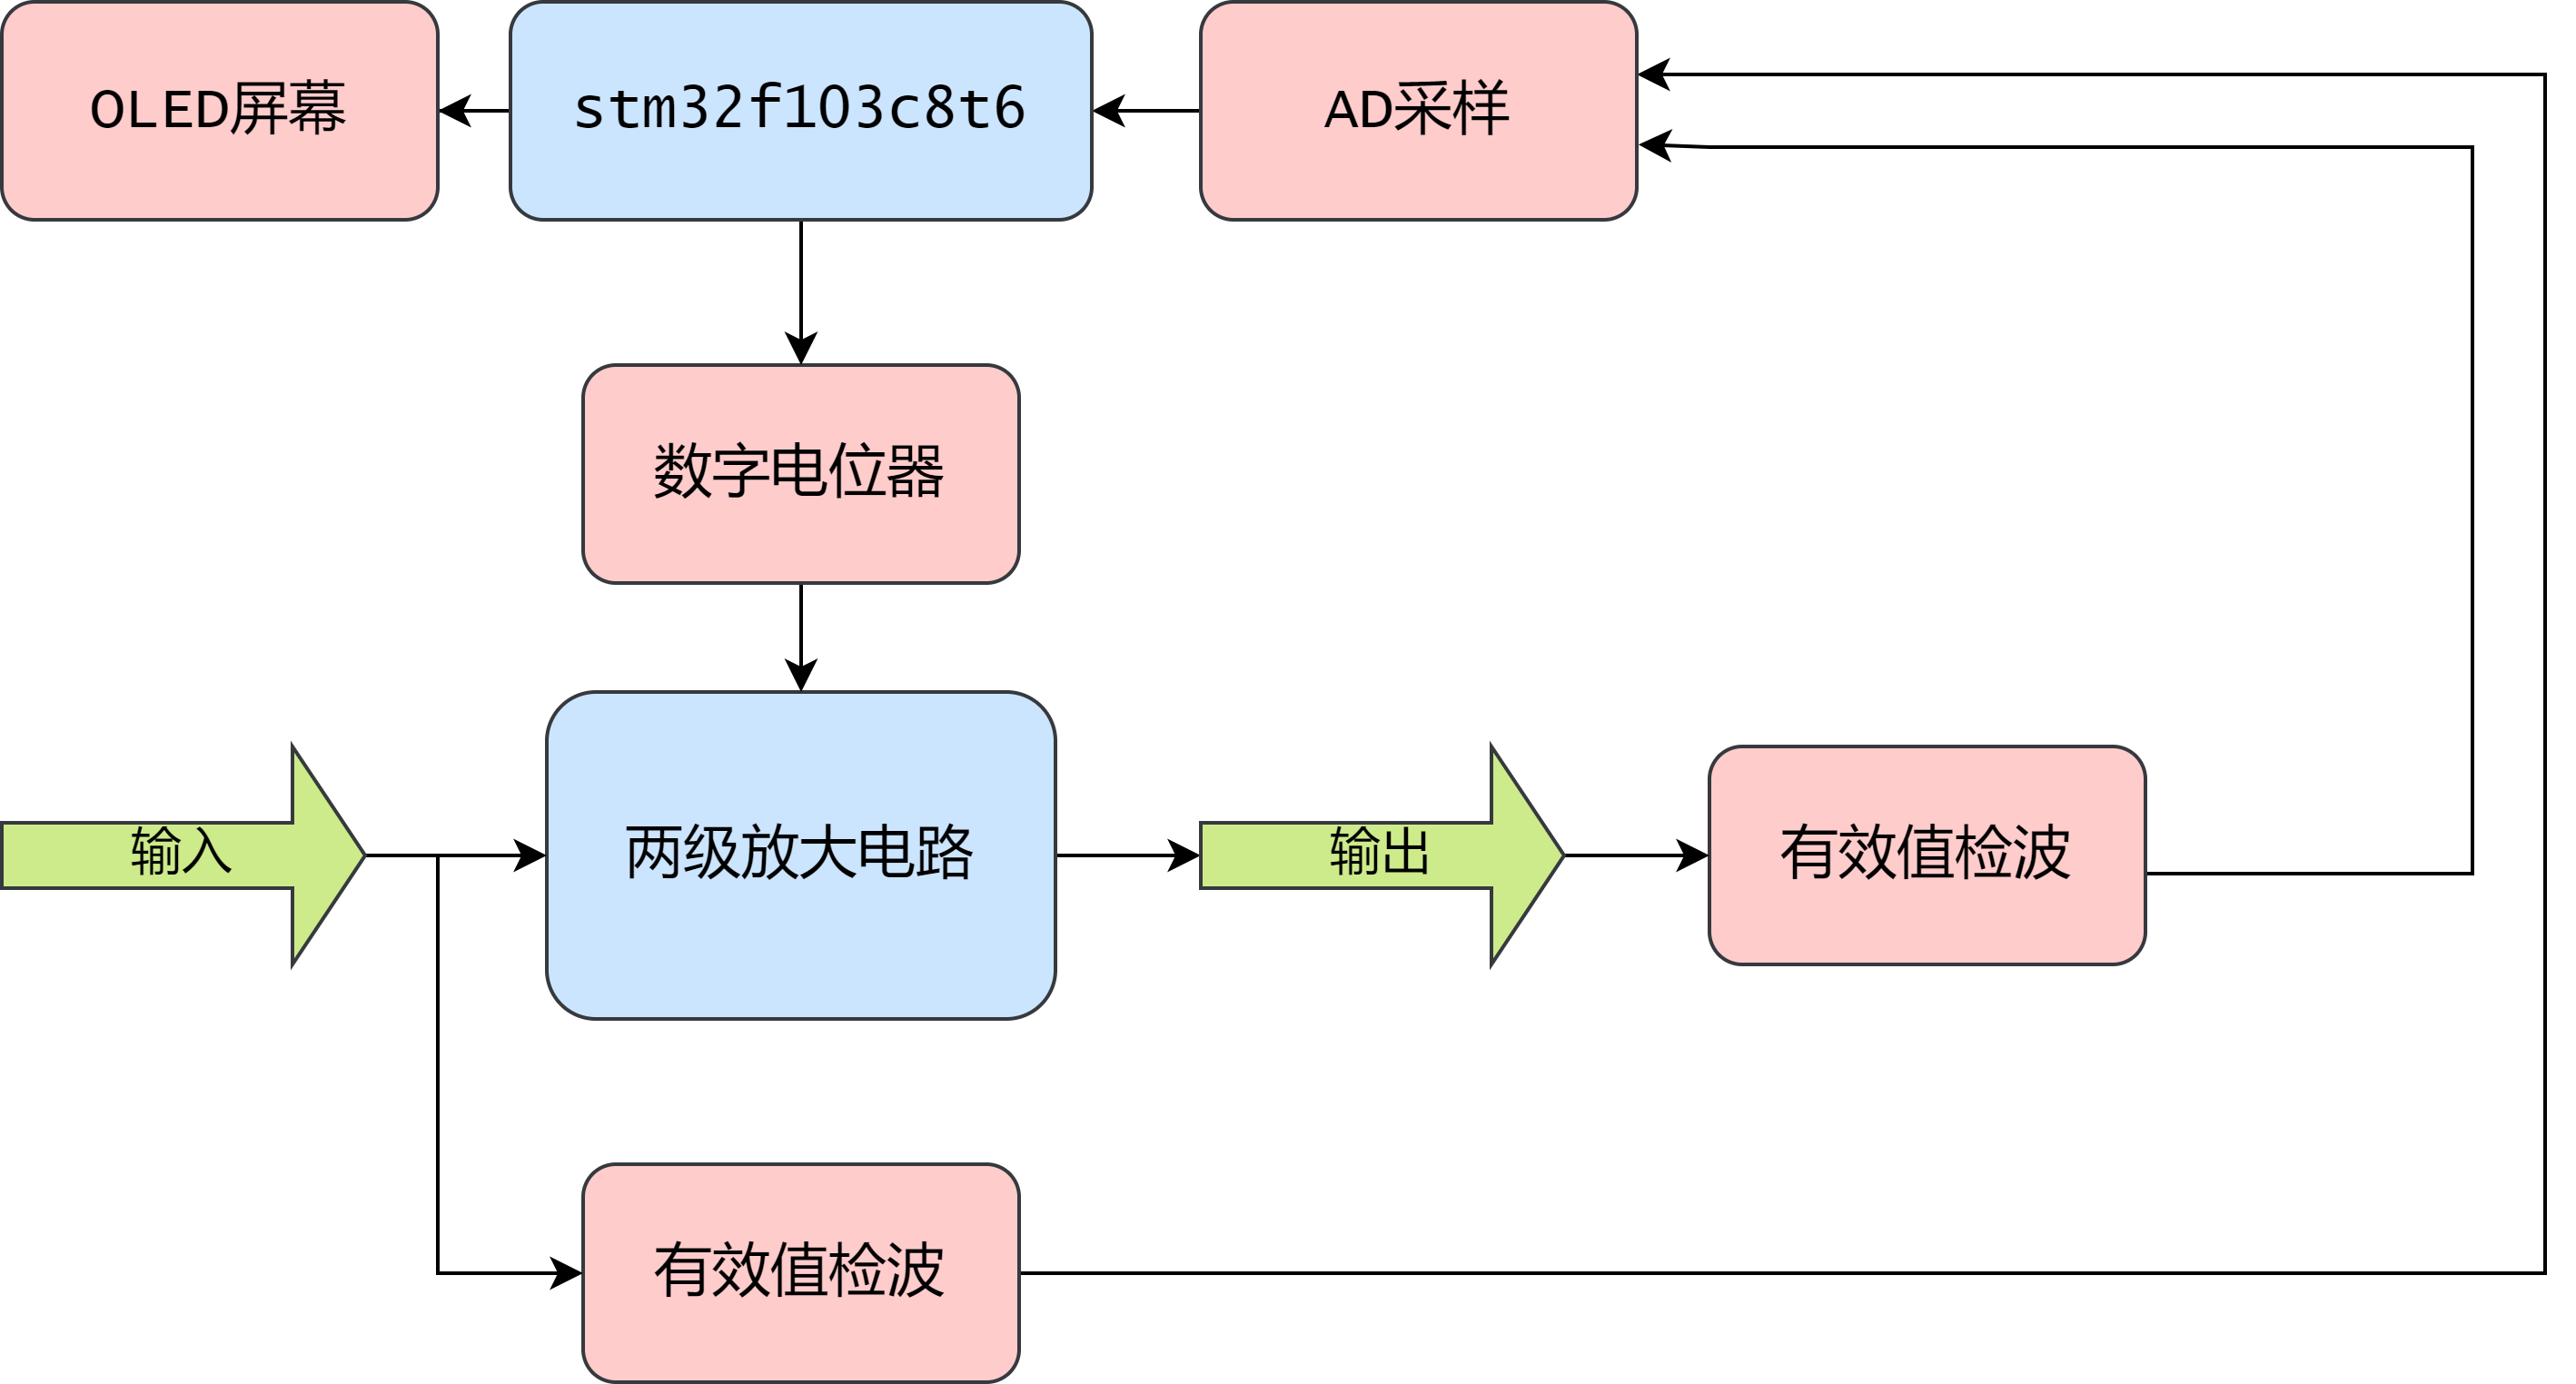
\includegraphics[width=1\textwidth]{硬件框图.png}
  \caption{硬件总体框图}
  \label{fig:hardware_picture}
\end{figure}
总体的硬件仿真图见附录1。

\subsection{可调两级反向放大电路}
该电路由三个运算放大器和数字电位器构成。一级运算放大器作为电压跟随器,来减少有效值检波与两级反向放大电路的干扰,并提高输入阻抗。后两级运算放大器(OPA2134)构成了反向放大电路,二级运算放大器的反馈电阻由数字电位器(AD5293)提供,通过调节数字电位器实现对该两级方向放大电路的放大倍数的调节,从而实现对输入信号的放大倍数的调节。如图 \ref{fig:two_stage_amplifier} 所示,该电路原理如下:

一级运算放大器的放大倍数为 \( -\frac{R_{17}}{R_{\text{数字电位器}}} \),二级运算放大器的放大倍数为 \( -\frac{R_{18}}{R_{19}} \)。因此,整个电路的放大倍数为:
\[
  \left( -\frac{R_{18}}{R_{19}} \right) \times \left( -\frac{R_{17}}{R_{\text{数字电位器}}} \right) = \frac{R_{18}}{R_{19}} \times \frac{R_{17}}{R_{\text{数字电位器}}}
\]

通过调节数字电位器的电阻值,可以调节电路的放大倍数。

由于市面上没有该型号的数字电位器模块,于是我们自行设计了数字电位器模块,原理图及PCB设计见附录2。
\begin{figure}[!htb]
  \centering
  \includegraphics[width=1\textwidth]{两级放大电路.png}
  \caption{可调两级放大电路 - proteus仿真}
  \label{fig:two_stage_amplifier}
\end{figure}

\subsection{有效值检波电路}
有效值检波电路的作用是将交流信号转换成直流信号,以解决题目中提高要求的 (2) 中的交流信号检测问题。

\begin{figure}[!htb]
  \centering
  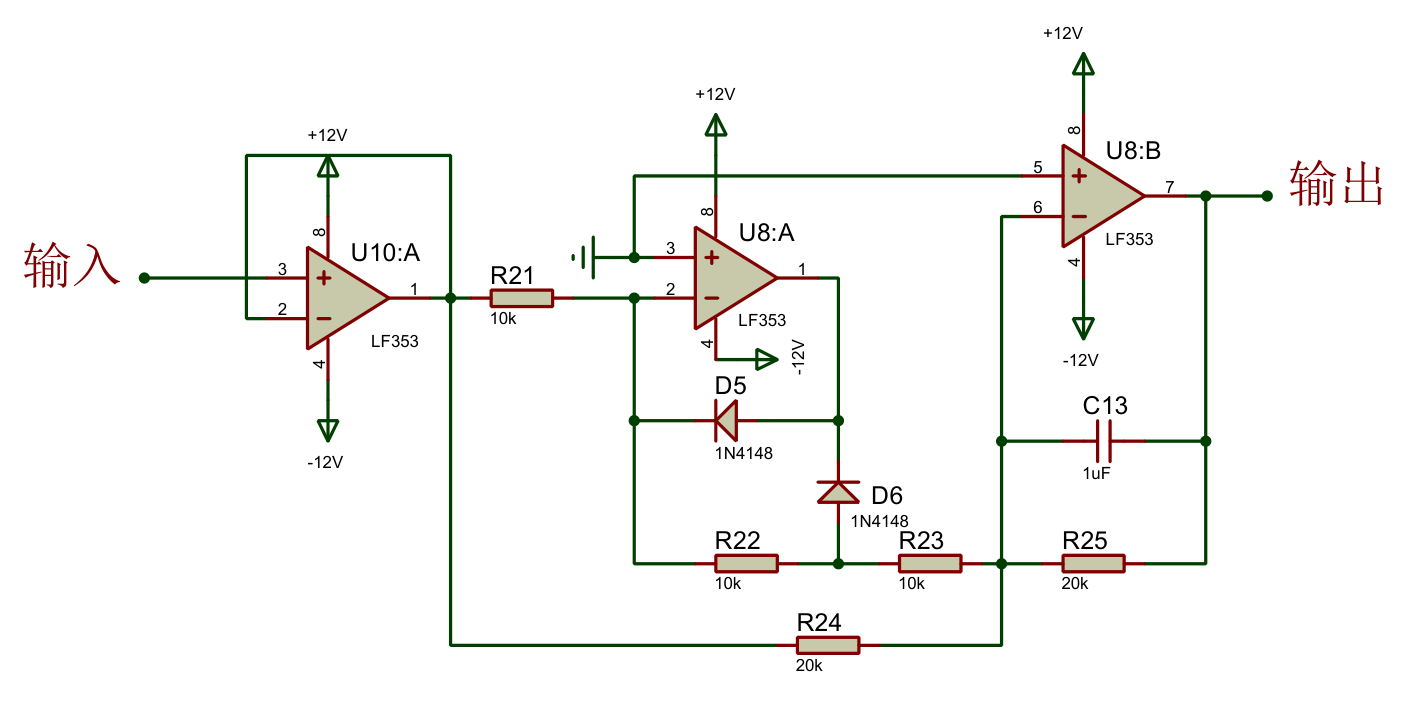
\includegraphics[width=1\textwidth]{有效值检波电路.png}
  \caption{有效值检波电路 - proteus仿真}
  \label{fig:effective_value_detection}
\end{figure}

如图\ref{fig:effective_value_detection}所示,该电路由三级运算放大器(LF353)和RC二极管检波网络构成,一级运算放大器作为电压跟随器,用于防止有效值检波电路与可调两级放大电路的相互干扰。

二级和三级运算放大器及RC二极管检波网络构成整流电路,完成有效值检波的功能。该电路原理如下:

(1) 当输入信号 \( U_i > 0 \) 时,二极管 \( D5 \) 截止,\( D6 \) 导通,此时一级运算放大器的增益为 \( -\frac{R_22}{R_21} = -1 \),所以 \( U_{o1} = -U_i \)。此时电路的输出信号 \( U_o \) 为:
\[
  U_o = -\frac{R_25}{R_24} U_i + \frac{R_25}{R_23} U_{o1} = U_i
\]

(2) 当输入信号 \( U_i < 0 \) 时,二极管 \( D5 \) 导通,\( D6 \) 截止,此时一级运算放大器的增益为 0,所以 \( U_{o1} = 0 \)。此时电路的输出信号 \( U_o \) 为:
\[
  U_o = -\frac{R_25}{R_24} U_i = -U_i
\]

由上所述,该电路可以实现整流功能。其中,电容 \( C1 \) 起到滤波作用。

\subsection{ADC采样模块}
由于STM32F103C8T6单片机的ADC模块只能采集0-3.3V的电压信号,而题目要求的最大电压为5V,因此我们外接了一个ADC进行电压信号的采集。如图\ref{fig:adc_sampling} 为ADC采样模块的展示。

\begin{figure}[!htb]
  \centering
  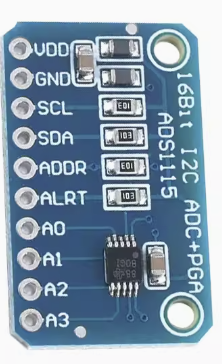
\includegraphics[width=0.25\textwidth]{ADC.png}
  \caption{ADC采样模块}
  \label{fig:adc_sampling}
\end{figure}

所使用的ADC为ADS1115,其是德州仪器推出的具有IIC接口的16位ADC转换器,超小型X2QFN或VSSOP封装,低功耗(20uA),宽电压输入2.0V-5.5V,可编程数据转换速率8SPS-860SPS,四个单端输入或两个差分输入。ADS1115具有内部低漂移基准源,支持单端或差分输入模式,可通过I2C接口进行编程。

\subsection{参数分析}
\subsubsection{带宽}
如下表\ref{tab:OPA2134}的所使用的放大器OPA2134的增益带宽积为8MHz,而根据题目要求可知AGC的最大增益为不会超过12倍,而最大频率100kHz下的增益带宽积为1.2MHz,所以满足题目要求。
\begin{table}[!ht]
  \centering
  \caption{OPA2134芯片参数}
  \begin{tabular}{|c|c|c|c|}
  \hline
      放大器类型 & 运算放大器 & 输入信号类型 & 差分  \\ \hline
      应用 & 音频设备 & 输出信号类型 & 差分  \\ \hline
      安装类型 & 通孔 & 典型增加带宽产品 & 8MHz  \\ \hline
      电源类型 & 双 & 最小CMRR & 86dB  \\ \hline
      每片芯片通道数目 & 2 & 最低工作温度 & -40°C  \\ \hline
      封装类型 & PDIP & 尺寸 & 9.81 x 6.35 x 4.57mm  \\ \hline
      引脚数目 & 8 & 最高工作温度 & +85°C \\ \hline
  \end{tabular}
  \label{tab:OPA2134}
\end{table}

\subsubsection{输入阻抗}
我们在电路输出端接入有一个电压跟随器,理论的输入电阻为无穷大,实测输入电阻为3MΩ,满足题目要求。


\subsubsection{输出阻抗}
查阅资料可知OPA2134的闭环输出阻抗为0.01Ω,开环输出阻抗为10Ω,本次采用两个OPA2134级联放大,估算可知不会超过1kΩ,满足题目要求。


\section{软件设计}

\subsection{AD采样}
\subsubsection{ADS1115简介}
ADS1115是德州仪器推出的具有IIC接口的16位ADC转换器,超小型X2QFN或VSSOP 封装,低功耗(20uA),宽电压输入2.0V-5.5V,可编程数据转换速率8SPS-860SPS,四个单端输入或两个差分输入。可应用于,电池电压电流检测,低速便携式仪表以及温度测量系统中。如图\ref{fig:ADS1115芯片结构}所示,为ADS1115芯片结构。
\begin{figure}[!htb]
  \centering
  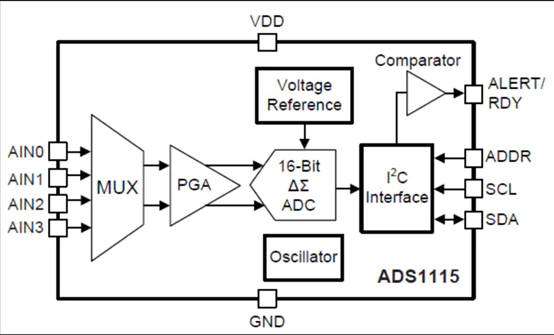
\includegraphics[width=0.7\textwidth]{ADS1115简介.png}
  \caption{ADS1115芯片结构}
  \label{fig:ADS1115芯片结构}
\end{figure}

如表\ref{tab:ADS1115引脚定义}所示,为ADS1115引脚定义。

\begin{table}[!ht]
  \centering
  \caption{ADS1115引脚定义}
  \begin{tabular}{ccc}
    \textbf{引脚名称} & \textbf{类型} & \textbf{描述 }   \\ \hline
    ADDR          & 数字量输入       & I2C 丛机地址选择     \\
    AIN0          & 模拟量输入       & 模拟量输入0通道       \\
    AIN1          & 模拟量输入       & 模拟量输入1通道       \\
    AIN2          & 模拟量输入       & 模拟量输入2通道       \\
    AIN3          & 模拟量输入       & 模拟量输入3通道       \\
    ALERT/RDY     & 数字量输出       & 比较器输出或转换就绪     \\
    GND           & 模拟量         & 接地             \\
    SCL           & 数字量输入       & IIC时钟          \\
    SDA           & 数字量输入/输出    & IIC数据线         \\
    VDD           & 模拟量         & VCC(2.0V-5.5V) \\
  \end{tabular}
  \label{tab:ADS1115引脚定义}
\end{table}

\subsubsection{通信方式}
ADS1115采用的是IIC通信。
\paragraph{IIC地址的选择}
ADS1115具有一个地址引脚ADDR,用于设置器件的I2C地址。 该引脚可以是连接到GND,VDD,SDA或SCL,因此可以通过一对IIC引脚选择四个不同的地址。

一般我们将地址位接GND,1001000,最后一位是确定IIC的写/读状态,写的时候是1,读的时候是0.所以slave address读写地址是0x90/0x91(10010000/10010001),如表\ref{tab:IIC}所示。

\begin{table}[!ht]
  \centering
  \caption{ADS1115的IIC地址}
  \begin{tabular}{cc}
    \textbf{ADDR PIN} & \textbf{SLAVE ADDRESS } \\ \hline
    Ground            & 1001000                 \\
    VDD               & 1001001                 \\
    SDA               & 1001010                 \\
    SCL               & 1001011                 \\
  \end{tabular}
  \label{tab:IIC}
\end{table}

\paragraph{接收模式}
ADS1115在从机接收模式下,主机发送到从机的第一个字节由7位设备地址组成,其次是低的R / W位。 主机发送的下一个字节是, ADS1115收到地址指针寄存器字节, 接下来的两个字节被写入地址由寄存器地址指针位P [1:0]给出。最后ADS1115返回字节。 数据寄存器字节为首先发送最高有效字节,然后发送最低有效字节。

\paragraph{发送模式}
在从机发送模式下,主机发送的第一个字节是7位从机地址,后跟高R / W位。 该字节将从机设置为发送模式, 从机发送的字节是数据寄存器的最高有效字节,由数据寄存器地址指针位P [1:0]指示, 然后,其余的最低有效字节由从机发送。

\subsubsection{ADS1115读写时序流程}
如图\ref{fig:IICTimeSequence}所示,为ADS1115读写时序流程。
\begin{figure}[!htb]
  \centering
  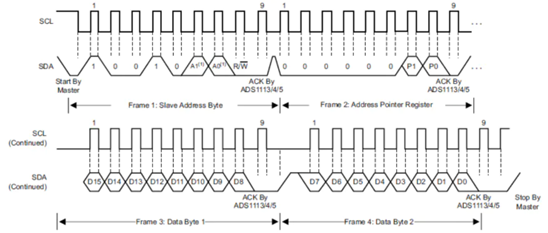
\includegraphics[width=1\textwidth]{IIC时序.png}
  \caption{ADS1115读写时序流}
  \label{fig:IICTimeSequence}
\end{figure}

\paragraph{读时序操作步骤}
\begin{enumerate}
  \item 发送写地址给 ADS1115 (0x90);
  \item 向地址指针寄存器写数据,后两位有效,只能写 0x00, 0x01, 0x02, 0x03;
  \item 发送读地址给 ADS1115 (0x91);
  \item 读取 ADS1115 的数据(两个字节,MSB 先行)。
\end{enumerate}

\paragraph{写时序操作步骤}
\begin{enumerate}
  \item 发送写地址给 ADS1115 (0x90);
  \item 向地址指针寄存器写数据,后两位有效,只能写 0x00, 0x01, 0x02, 0x03;
  \item 发送数据给 ADS1115(高位在前)。
\end{enumerate}

\subsubsection{ADS1115输出数据格式}
ADS1115以二进制补码格式提供16位数据。 正满量程(+ FS)输入时,输出的AD值代码为7FFFh,负满量程(-FS)输入时,输出的AD值代码为8000h。这些代码的输出为了提示超量程的提示。

\subsubsection{程序流程图}
如图\ref{fig:ADS1115程序流程图}所示,为ADS1115程序流程图。首先初始化IIC,然后读取范围,之后读取ADS1115的数据,最后将数据转换为电压值的小数显示。
\begin{figure}[!htb]
  \centering
  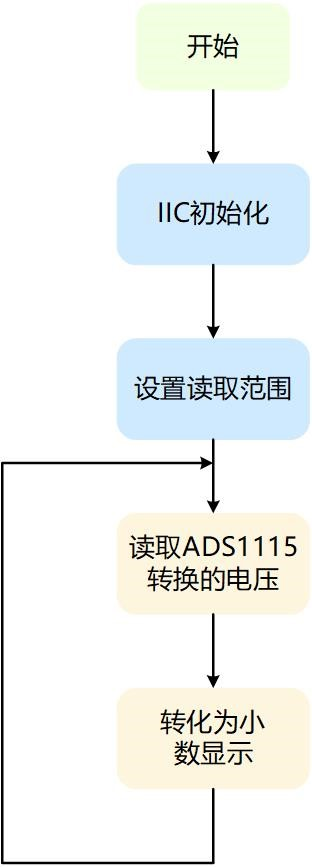
\includegraphics[width=0.3\textwidth]{ADS1115程序流程图.jpg}
  \caption{ADS1115程序流程图}
  \label{fig:ADS1115程序流程图}
\end{figure}

\subsection{数字电位器}
\subsubsection{AD5293简介}
AD5293是一款单通道、1024位数字电位计1 ,端到端电阻容差<1\%。该器件可实现与机械电位计相同的电子调整功能,而且具有增强的分辨率、固态可靠性和出色的低温度系数性能。它可在高电压下工作,既可采用±10.5 V至±15 V双电源供电,也可采用21 V至33 V单电源供电。MCU通过SPI方式与其通信。如图\ref{fig:ad5293芯片结构}所示,为AD5293芯片结构。
\subsubsection{程序流程图}
\begin{figure}[!htb]
  \centering
  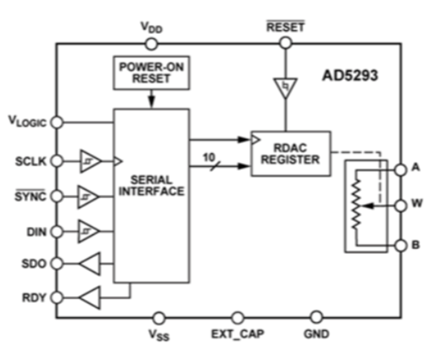
\includegraphics[width=0.5\textwidth]{ad5293芯片结构.png}
  \caption{AD5293芯片结构}
  \label{fig:ad5293芯片结构}
\end{figure}

\subsubsection{AD5293通信}
AD5293采用的是标准的SPI通信。
\subsubsection{SPI通信简介}
SPI接口主要应用在EEPROM、FLASH、实时时钟、AD转换器,还有数字信号处理器和数字信号解码器之间。SPI是一种高速的,全双工,同步的通信总线,并且在芯片的管脚上只占用四根线,节约了芯片的管脚,同时为PCB的布局上节省空间,提供方便,正是出于这种简单易用的特性,现在越来越多的芯片集成了这种通信协议,比如AT91RM9200。

SPI分为主、从两种模式,一个SPI通讯系统需要包含一个(且只能是一个)主设备,一个或多个从设备。SPI接口的读写操作,都是由主设备发起。当存在多个从设备时,通过各自的片选信号进行管理。

\subsubsection{引脚说明}
SPI的通信原理很简单,它以主从方式工作,这种模式通常有一个主设备和一个或多个从设备,需要至少4根线,事实上3根也可以(单向传输时)。这四根线分别是MISO、MOSI、SCLK、CS,具体的描述见下表\ref{tab:SPI}:
\begin{table}[!ht]
  \centering
  \caption{SPI引脚说明}
  \begin{tabular}{cc}
    \textbf{名称} & \textbf{描述 }    \\ \hline
    MISO        & 主设备数据输出,从设备数据输入 \\
    MOSI        & 主设备数据输出,从设备数据输入 \\
    SCLK        & 时钟信号,主设备产生      \\
    CS          & 片选信号,主设备控制      \\
  \end{tabular}
  \label{tab:SPI}
\end{table}

\subsubsection{程序流程图}
如图\ref{fig:AD5293程序流程图}所示,为AD5293程序流程图。首先初始化AD5293,之后通过SPI通信方式与AD5293通信,进行片选和读写操作。

\begin{figure}[!htb]
  \centering
  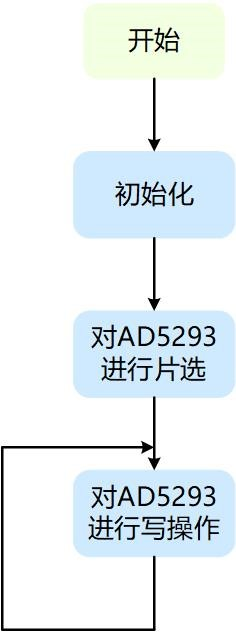
\includegraphics[width=0.2\textwidth]{AD5293程序流程图.jpg}
  \caption{AD5293程序流程图}
  \label{fig:AD5293程序流程图}
\end{figure}

\subsection{主程序}
\subsubsection{主程序介绍}
如图\ref{fig:主程序流程图}主程序用来初始化各种外设,以及对整个硬件电路的逻辑编写。初始化ADS1115,OLED以及AD5293等外设之后,进入到按键检测,根据不同的按键按下来切换到不同的模式从而达到所需的要求。

\subsubsection{主程序流程图}
\begin{figure}[!htb]
  \centering
  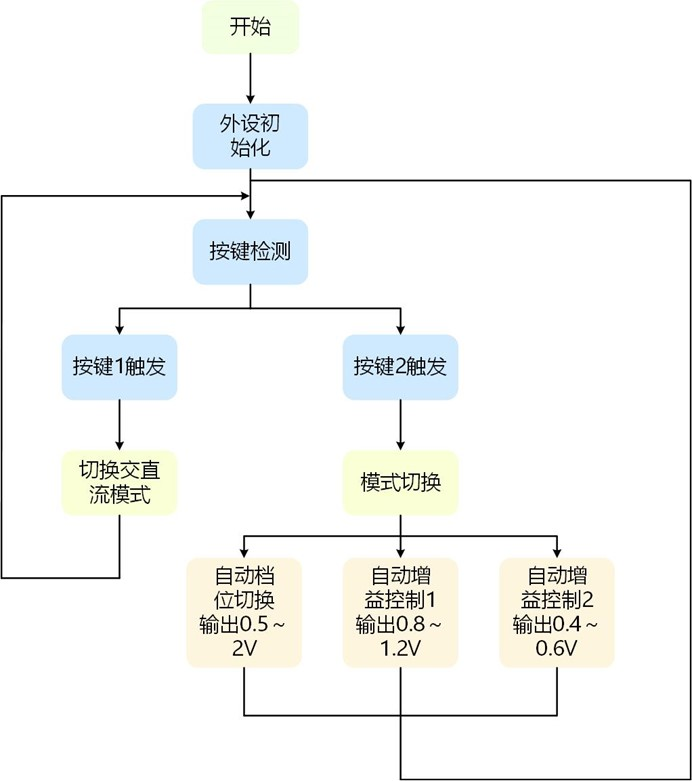
\includegraphics[width=0.7\textwidth]{主程序.jpg}
  \caption{主程序流程图}
  \label{fig:主程序流程图}
\end{figure}

其中自动控制模式下的输出电压范围控制采用的是和ADC转换原理类似的逐次逼近比较,从而让他限定在所需的输出范围内。部分代码呈现如下:
\begin{lstlisting}[language=C,caption={主程序部分代码},label={code:zhu}]
void just_vol(float vol_ref,float vol,float output_singal)
{
    if((output_singal >vol_ref)&&((output_singal-vol_ref)>vol))
    {
        AD5293_Write(write,i--);
        if(i<=0x0001)
        i=0x0002:
      }
    else if((output_singal <vol_ref)&&((vol_ref output_singal)>vol))
    {
        AD5293_Write(write,i ++)
        if(i>=0x3FFF){
            i=0x3FFE:
          }
      }
  }
  \end{lstlisting}
其中 vol\_ref代表为基准电压,vol代表为允许的最大误差,output\_singal为输出的电压。

\section{系统测试}

\subsection{测试概述}
\begin{enumerate}
  \item 测试目的:评估该自动增益控制系统的质量、可靠性、安全性和性能。

  \item 测试范围:包括所有的功能、性能和安全性测试。

  \item 测试工具:

        使用以下工具进行测试,
        \begin{enumerate}
          \item \textbf{可调直流源和信号发生器}:用于提供测试的输入信号。
          \item \textbf{实验箱和自制电源电路}:为系统中的芯片供电。
          \item \textbf{电压表}:用于检测和调试电路中的信号。
        \end{enumerate}

\end{enumerate}

\subsection{基本要求(1)}
系统设置有0.2、 0.5、 2、 5 四挡增益,通过按键1可以对档位进行切换。本次进行三次测试,规定输入直流信号的大小为0.1V、1V、2V,分别测试系统在四挡增益下的输出电压。

当输入直流信号为0.1V时,系统测试如表\ref{tab:1_0.1V}所示。
\begin{table}[!ht]
  \centering
  \caption{基本要求(1)测试结果(输入为0.1V时)}
  \begin{tabular}{cccccc}
    \textbf{按键按下次序} & \textbf{电压表测量输入信号(V)} & \textbf{电压表测量输出信号(V)} & \textbf{理论增益} & \textbf{实际增益} & \textbf{测试是否通过} \\ \hline
    0               & 0.10                  & 0.02                  & 0.2           & 0.2           & 通过              \\
    1               & 0.10                  & 0.05                  & 0.5           & 0.5           & 通过              \\
    2               & 0.11                  & 0.21                  & 2             & 2             & 通过              \\
    4               & 0.10                  & 0.49                  & 5             & 5             & 通过              \\
    5               & 0.10                  & 0.02                  & 0.2           & 0.2           & 通过              \\
    6               & 0.10                  & 0.05                  & 0.5           & 0.5           & 通过              \\
    7               & 0.10                  & 0.20                  & 2             & 2             & 通过              \\
    8               & 0.10                  & 0.49                  & 5             & 4.9           & 通过              \\
    9               & 0.10                  & 0.02                  & 0.2           & 0.2           & 通过              \\
    10              & 0.10                  & 0.05                  & 0.5           & 0.5           & 通过              \\
    11              & 0.10                  & 0.21                  & 2             & 2.1           & 通过              \\
    12              & 0.10                  & 0.49                  & 5             & 4.9           & 通过              \\
  \end{tabular}
  \label{tab:1_0.1V}
\end{table}

当输入直流信号为1V时,系统测试如表\ref{tab:1_1V}所示。
\begin{table}[!ht]
  \centering
  \caption{基本要求(1)测试结果(输入为1V时)}
  \begin{tabular}{cccccc}
    \textbf{按键按下次序} & \textbf{电压表测量输入信号(V)} & \textbf{电压表测量输出信号(V)} & \textbf{理论增益} & \textbf{实际增益} & \textbf{测试是否通过} \\ \hline
    0               & 1.01                  & 0.20                  & 0.2           & 0.2           & 通过              \\
    1               & 1.01                  & 0.51                  & 0.5           & 0.5           & 通过              \\
    2               & 1.02                  & 2.03                  & 2             & 2             & 通过              \\
    4               & 1.01                  & 5.00                  & 5             & 5             & 通过              \\
    5               & 1.01                  & 0.20                  & 0.2           & 0.2           & 通过              \\
    6               & 1.01                  & 0.51                  & 0.5           & 0.5           & 通过              \\
    7               & 1.02                  & 2.03                  & 2             & 2             & 通过              \\
    8               & 1.00                  & 5.02                  & 5             & 5             & 通过              \\
    9               & 1.01                  & 0.21                  & 0.2           & 0.2           & 通过              \\
    10              & 1.00                  & 0.51                  & 0.5           & 0.5           & 通过              \\
    11              & 1.02                  & 2.05                  & 2             & 2             & 通过              \\
    12              & 1.01                  & 5.01                  & 5             & 5             & 通过              \\
  \end{tabular}
  \label{tab:1_1V}
\end{table}

当输入直流信号为2V时,系统测试如表\ref{tab:1_2V}所示。
\begin{table}[!ht]
  \centering
  \caption{基本要求(1)测试结果(输入为2V时)}
  \begin{tabular}{cccccc}
    \textbf{按键按下次序} & \textbf{电压表测量输入信号(V)} & \textbf{电压表测量输出信号(V)} & \textbf{理论增益} & \textbf{实际增益} & \textbf{测试是否通过} \\ \hline
    0               & 2.00                  & 0.42                  & 0.2           & 0.2           & 通过              \\
    1               & 2.01                  & 1.03                  & 0.5           & 0.5           & 通过              \\
    2               & 2.03                  & 4.02                  & 2             & 2             & 通过              \\
    4               & 2.03                  & 9.98                  & 5             & 5             & 通过              \\
    5               & 2.01                  & 0.41                  & 0.2           & 0.2           & 通过              \\
    6               & 2.00                  & 1.01                  & 0.5           & 0.5           & 通过              \\
    7               & 2.01                  & 4.01                  & 2             & 2             & 通过              \\
    8               & 2.01                  & 10.00                 & 5             & 5             & 通过              \\
    9               & 2.01                  & 0.41                  & 0.2           & 0.2           & 通过              \\
    10              & 2.01                  & 1.00                  & 0.5           & 0.5           & 通过              \\
    11              & 2.01                  & 4.01                  & 2             & 2             & 通过              \\
    12              & 2.02                  & 10.03                 & 5             & 5             & 通过              \\
  \end{tabular}
  \label{tab:1_2V}
\end{table}

输出信号与实际增益在误差允许的范围内,均符合理论值,测试通过。
\subsection{基本要求(2)}
使用0.96寸的OLED显示屏,显示输出和输出信号的幅度当前放大器的增益。
显示的内容为:\textbf{ADC0:X.XXXX,ADC1:X.XXXX, amp:X.XXXX}。其中ADC0为输入信号的幅度,ADC1为输出信号的幅度,amp为当前放大器的增益。显示的数值大小均为实际测量值,保留四位小数。

本次进行三次测试,规定输入直流信号的大小为0.1V、1V、2V,观察OLED显示屏上的显示结果是否与电压表测量值一致,及增益是否与电路设计值一致。测试结果如表\ref{tab:2_OLED}所示。
\begin{table}[!ht]
  \centering
  \caption{基本要求(2)测试结果}
  \begin{tabular}{cccc}
    \diagbox{名称}{序号} & \textbf{1} & \textbf{2} & \textbf{3} \\ \hline
    输入信号幅度(V)        & 0.1        & 1          & 2          \\
    电压表测量输入信号幅度(V)   & 0.12       & 1.01       & 2.03       \\
    电压表测量输出信号幅度(V)   & 0.25       & 5.08       & 1.01       \\
    OLED显示输入信号幅度(V)  & 0.1217     & 1.0125     & 2.0315     \\
    OLED显示输入信号幅度(V)  & 0.2514     & 5.0832     & 1.0122     \\
    OLED显示增益         & 2.0657     & 5.0204     & 0.4982     \\
    理论增益             & 2          & 5          & 0.5        \\
    显示是否正常           & 正常         & 正常         & 正常         \\
  \end{tabular}
  \label{tab:2_OLED}
\end{table}
显示屏在测试中均正常显示,显示值与测量值在误差允许的范围内,符合理论值,显示结果正确,测试通过。
\subsection{基本要求(3)与提高要求(1)}
考虑到基本要求(3)与提高要求(1)的测试内容相似,测试指标重合,因此将两者合并进行测试。本次进行六次测试,规定输入直流信号的大小为0.1V、1V、2V、3V、4V、5V。测试结果如表\ref{tab:3_1}所示。
\begin{table}[!ht]
  \centering
  \caption{基本要求(2)与提高要求(1)的测试结果}
  \begin{tabular}{ccccccc}
    \textbf{输入信号(V)} & \textbf{0.10} & \textbf{1.2} & \textbf{2.4} & \textbf{3.3} & \textbf{4.5} & \textbf{5} \\ \hline
    ADC0(OLED)       & 0.1035        & 1.2065       & 2.4079       & 3.3721       & 4.5890       & 5.0690     \\
    ADC1(OLED)       & 1.1653        & 1.1431       & 1.1733       & 1.1711       & 0.9832       & 0.9911     \\
    Amp(OLED)        & 11.2589       & 0.9803       & 0.4872       & 0.3473       & 0.2142       & 0.1955     \\
    测量输入信号(V)        & 0.10          & 1.20         & 2.40         & 3.37         & 4.58         & 5.06       \\
    测量输出信号(V)        & 1.16          & 1.14         & 1.17         & 1.17         & 0.98         & 0.99       \\
    测量增益             & 11.25         & 0.98         & 0.48         & 0.34         & 0.21         & 0.19       \\
    0.5\~2V(是否)      & 是             & 是            & 是            & 是            & 是            & 是          \\
    0.8\~2V(是否)      & 是             & 是            & 是            & 是            & 是            & 是          \\
  \end{tabular}
  \label{tab:3_1}
\end{table}
测试结果显示,输出信号、实际增益和显示屏显示内容在误差允许的范围内,均符合理论值,测试通过。

值得注意的是,我们发现显示屏上显示的输入信号与信号源输入的信号有一直存在较为明显的误差,为0.0XV,起初我们认为是ADC采样模块的问题,但经过多次测试,我们发现ADC采样模块的采样值是准确的,因此我们怀疑是OLED显示屏的问题。经过查阅资料,我们发现OLED显示屏的显示值是由其内部的ADC采样模块采样得到的,因此我们认为OLED显示屏的显示值是准确的。之后我们怀疑是电压表的问题,于是我们对电压表进行了校准,误差依然存在。我们又尝试直接对信号源输入的信号进行了测量,发现信号源本身的输出电源不准确。

\subsection{提高要求(2)}
本次进行了六次测试,规定输入信号的幅度为0.2V、2.4V、2V、4.8V、6.6V、9V、10V,输入信号的频率对应3kHz、10kHz、30kHz、50kHz、70kHz、100kHz。测试结果如表\ref{tab:4_2}所示。

\begin{table}[!ht]
  \centering
  \caption{提高要求(2)的测试结果}
  \begin{tabular}{ccccccc}
    \textbf{输入信号幅度(Vpp)(V)} & \textbf{0.20} & \textbf{2.4} & \textbf{4.8} & \textbf{6.6} & \textbf{9} & \textbf{10} \\ \hline
    输入信号频率(kHz)             & 3             & 10           & 30           & 50           & 70         & 100         \\
    ADC0(OLED)              & 0.1045        & 1.2030       & 2.4088       & 3.3755       & 4.5855     & 5.0678      \\
    ADC1(OLED)              & 1.1615        & 1.1455       & 1.1778       & 1.1735       & 0.9857     & 0.9954      \\
    Amp(OLED)               & 11.1148       & 0.9522       & 0.4889       & 0.3476       & 0.2149     & 0.1964      \\
    测量输入信号(V)               & 0.10          & 1.20         & 2.40         & 3.37         & 4.58       & 5.06        \\
    测量输出信号(V)               & 1.16          & 1.14         & 1.17         & 1.17         & 0.98       & 0.99        \\
    测量增益                    & 11.60         & 0.95         & 0.48         & 0.34         & 0.21       & 0.19        \\
    0.8\~1.2(Vpp)(是否)       & 是             & 是            & 是            & 是            & 是          & 是           \\
  \end{tabular}
  \label{tab:4_2}
\end{table}
由于显示屏和电压表显示的是Vp值,所以其值是Vpp的二分之一。测试结果显示,输出信号、实际增益和显示屏显示内容在误差允许的范围内,均符合理论值,测试通过。

值得注意的是,本电路在100kHz的高频下,仍然能保持较好的自动增益控制效果,未出现因频率过高导致的衰减现象。与此相比,网上很多AGC电路设计都会出现频率过高导致的衰减现象,本设计的电路在高频下仍然能保持较好的自动增益控制效果,具有较好的性能。

\section{总结}
本设计实现了一个自动增益控制系统,能够自动调节输入信号的放大倍数,使输出信号的幅度保持在合适的范围内。系统硬件设计合理,性能稳定,满足了设计要求。经过系统测试,系统的功能、性能和安全性均符合要求,测试结果良好,验证了系统的可靠性和稳定性。

在测试过程中,我们发现了一些问题。

输入信号的幅度与信号源的输出信号存在较大误差,经过多次测试,我们发现是信号源本身的问题。在今后的设计中,我们需要更加注意信号源的准确性,以保证测试结果的准确性。

在初次测试中我们发现电路输出异常,经过对焊接和电路设计的排查后,我们发现是电路没有“共地”,整体的电路的所有的GND与电源的GND要联通,否则会导致电路不工作或者输入出现问题,对电路影响很大。

\begin{thebibliography}{99} % 如果你的文献数量超过 9 条,使用 {99} 可以确保正确对齐
  \bibitem{perez2011automatic}
  Juan Pablo Alegre Pérez, Santiago Celma Pueyo, Belén Calvo López.
  \textit{Automatic gain control}.
  Springer, 2011.

  \bibitem{ohlson1974exact}
  J. Ohlson.
  \textit{Exact dynamics of automatic gain control}.
  \textit{IEEE Transactions on Communications}, 22(1):72--75, 1974.

  \bibitem{martinez2001automatic}
  Isaac Martinez.
  \textit{Automatic gain control (AGC) circuits theory and design}.
  Term paper, University of Toronto, 2001.

  \bibitem{lu2023}
  卢霄.
  \textit{一种延迟式自动增益控制电路的设计及仿真研究}.
  \textit{电子制作}, 18:83--85+78, 2023.

  \bibitem{lu2023}
  卢霄.
  \textit{声系统设备第8部分: 自动增益控制装置}.
  \textit{中华人民共和国电子工业部}, SJ/Z 9140.3-1987, 1987.


  \bibitem{按键}
  \textit{stm32f103——外部中断和事件——检测按键按下点灯}.
  \url{https://blog.csdn.net/qq_39577221/article/details/125304686}.

  \bibitem{按键}
  \textit{运放的参数详解及应用电路}.
  \url{https://blog.csdn.net/qq_21794157/article/details/124024270}.

  \bibitem{按键}
  \textit{可变增益放大器电路VCA电路,自动增益控制电路AGC电路}.
  \url{https://www.bilibili.com/video/BV1JD4y1b7Gzvd_source=565626543e6250b5a2589e84e31771f6}.

  \bibitem{按键}
  \textit{增益自动切换电压放大电路设计}.
  \url{https://blog.csdn.net/weixin_45012516/article/details/109273168}.

  \bibitem{按键}
  \textit{基于VCA821的AGC,电压自动增益控制设计}.
  \url{https://zhuanlan.zhihu.com/p/644879914}.
\end{thebibliography}



\begin{appendices}
  \section{附录1 - 硬件总体仿真电路图(proteus仿真)}
  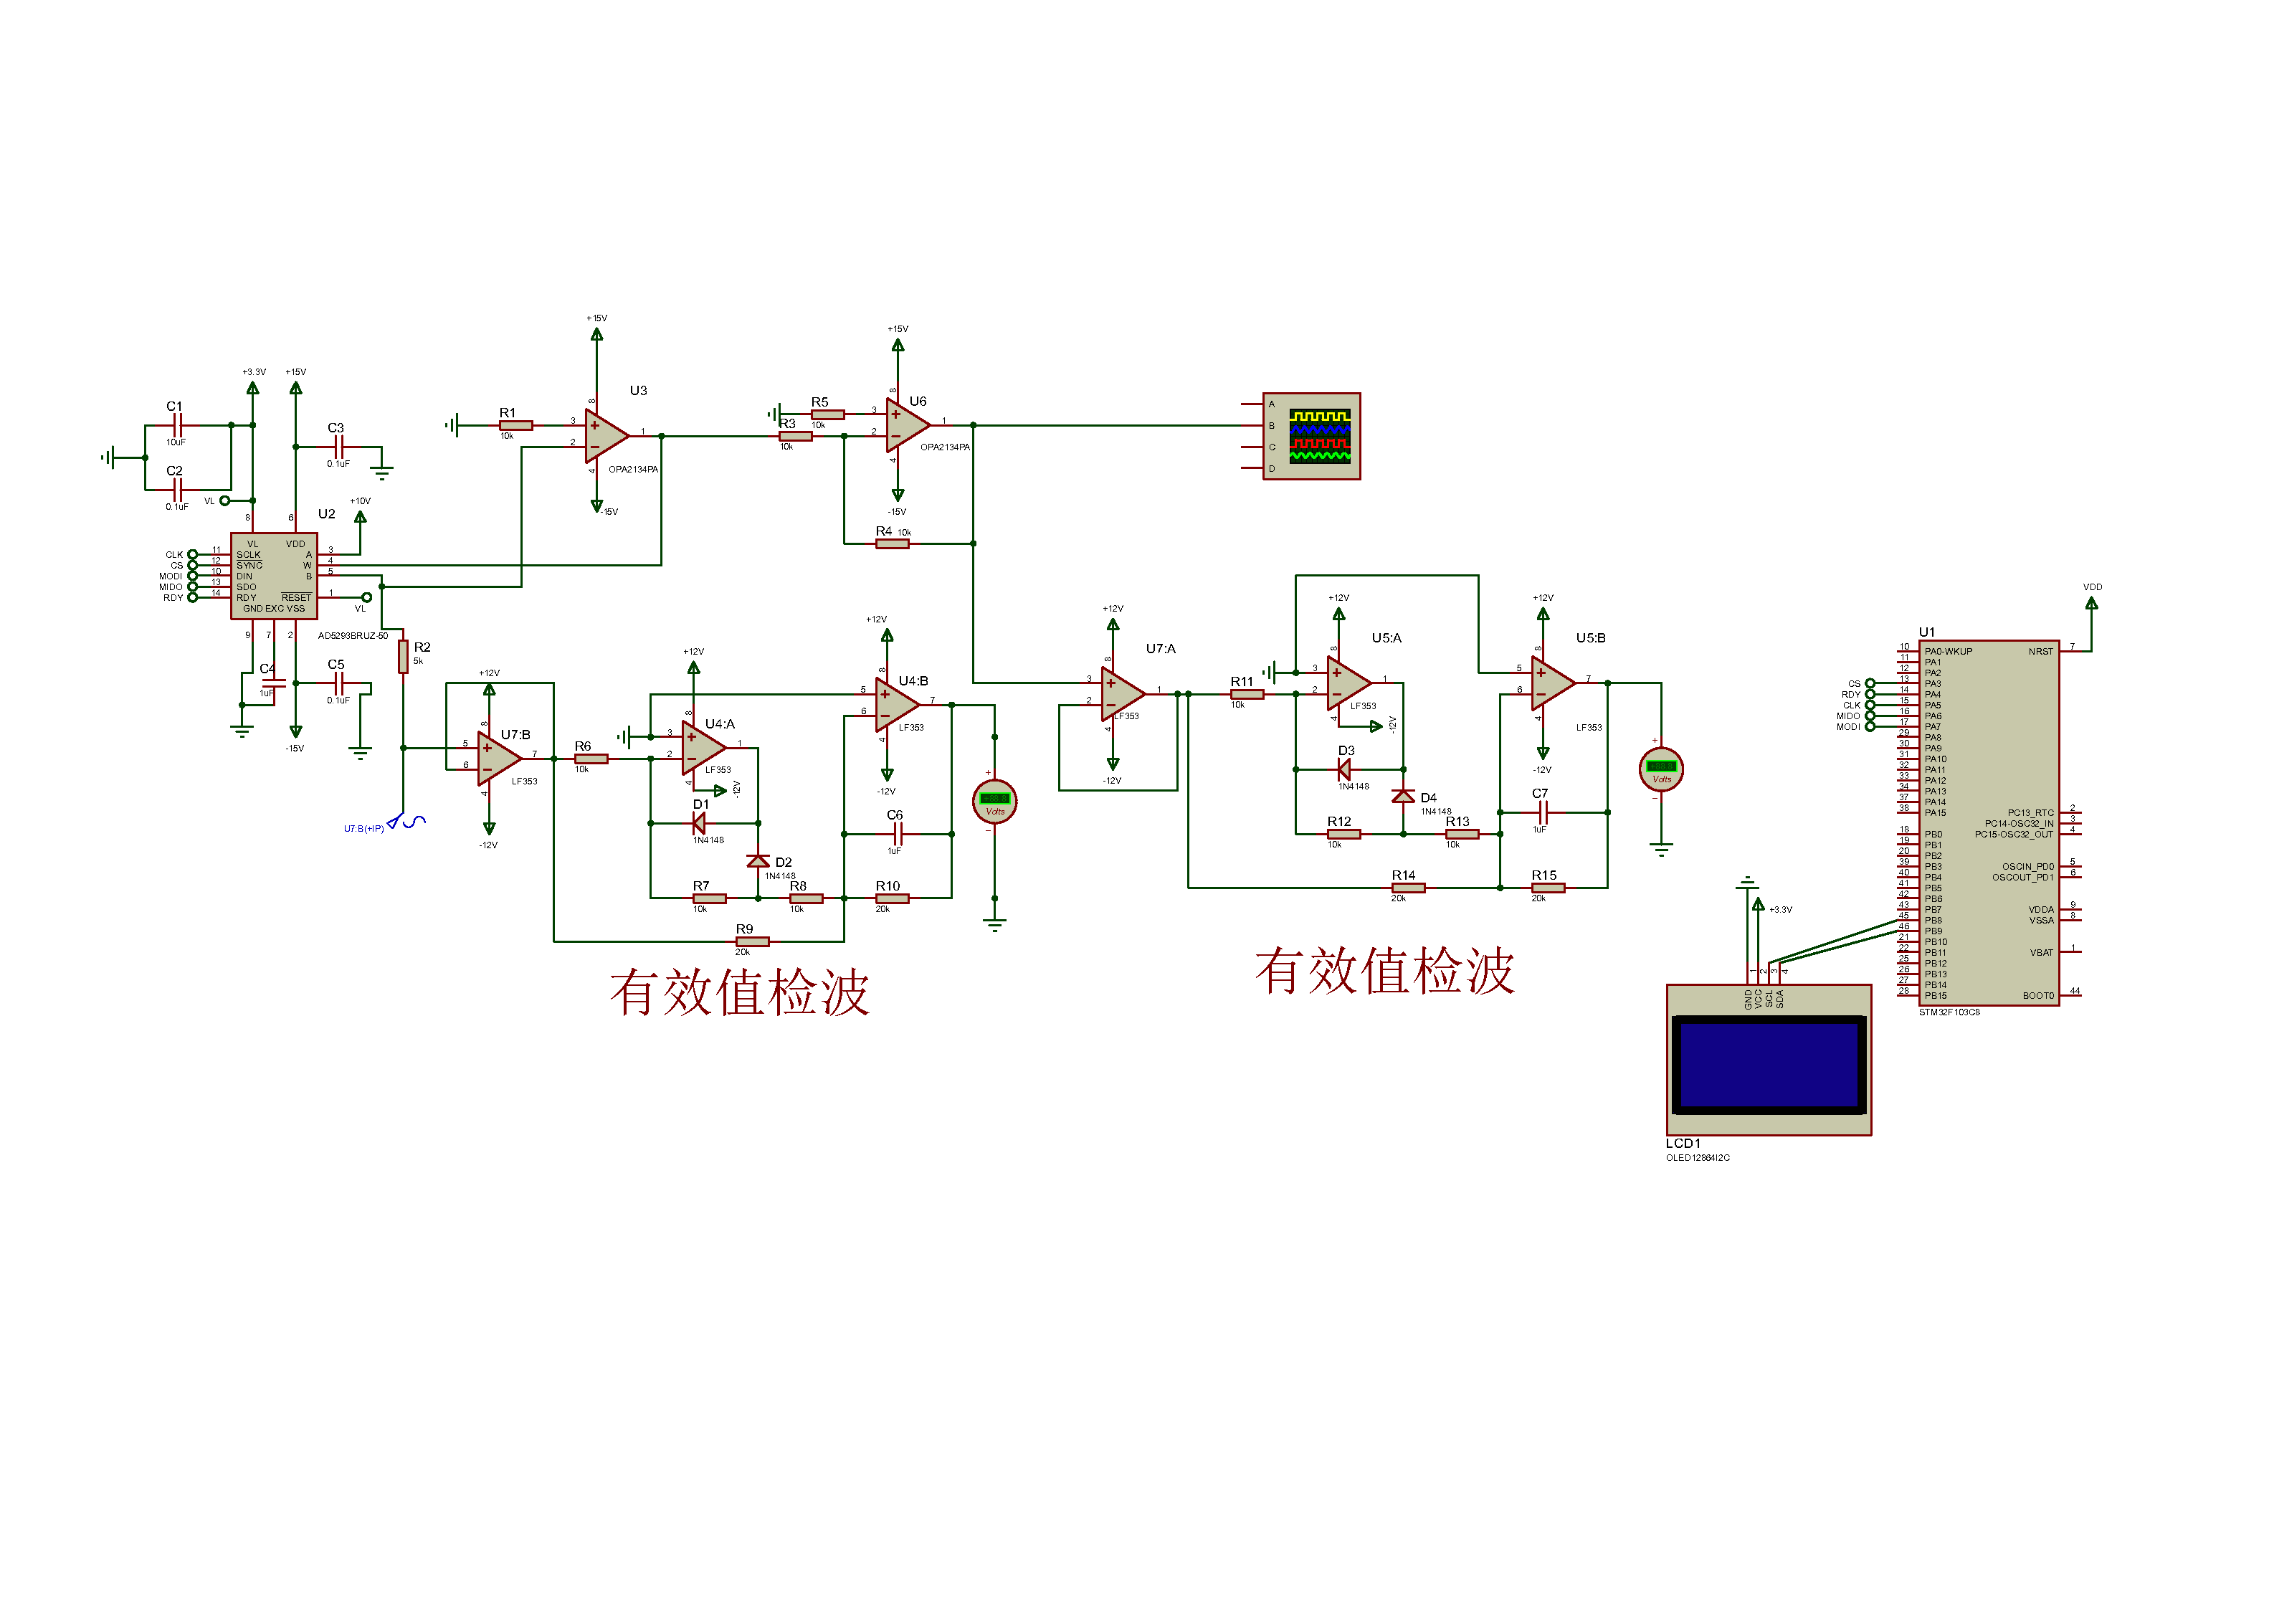
\includepdf[pages=-,angle=90]{数字电位器真1.pdf}

  \section{附录2 - 数字电位器的原理图及PCB}
  \begin{figure}[!htb]
    \centering
    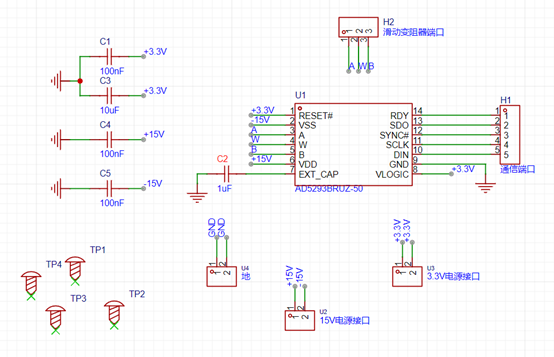
\includegraphics[width=0.8\textwidth]{数字电位器原理图.png}
    \caption{数字电位器原理图}
    \label{fig:数字电位器原理图}
  \end{figure}

  \begin{figure}[H]
    \centering
    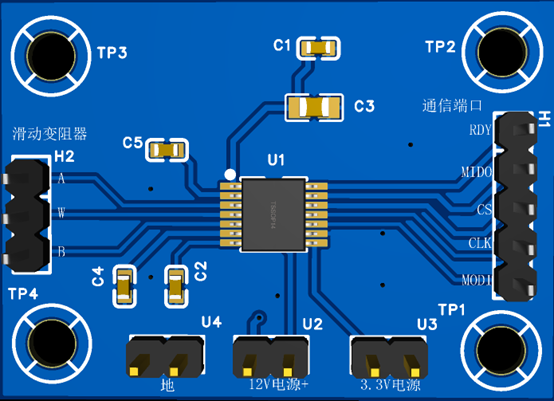
\includegraphics[width=0.9\textwidth]{PCB正面.png}
    \caption{数字电位器PCB正面}
    \label{fig:PCB正面}
  \end{figure}

  \begin{figure}[H]
    \centering
    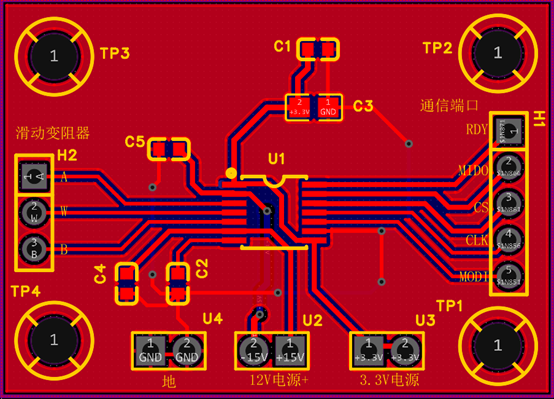
\includegraphics[width=0.9\textwidth]{PCB背面.png}
    \caption{数字电位器PCB背面}
    \label{fig:PCB背面}
  \end{figure}

  \section{附录3 - main.c}
  \lstinputlisting[caption={main.c}, label={lst:main.c}]{code/main.c}
\end{appendices}

\end{document}
